%%%%%%%%%%%%%%%%%%%%%%%%%%%%%%%%%%%%%%%%%%%%%%%%%%%%%%%%%%%%%%%%%%%%%%%%%%%%%%%%
%%% Results
%%%%%%%%%%%%%%%%%%%%%%%%%%%%%%%%%%%%%%%%%%%%%%%%%%%%%%%%%%%%%%%%%%%%%%%%%%%%%%%%

\clearpage
\section{Discussion}
\label{sec:discussion}

\subsection{Results}

%T\"ass\"a osassa esitet\"a\"an tulokset ja vastataan tutkielman alussa
%esitettyihin tutkimuskysymyksiin. Tieteellisen kirjoitelman
%arvo mitataan t\"ass\"a osassa esitettyjen tulosten perusteella.

\nyi{Graphs generated by the system (pictures!)}

% conforming to the JSON graphs (visually?)

\begin{figure}[htb]
\centering 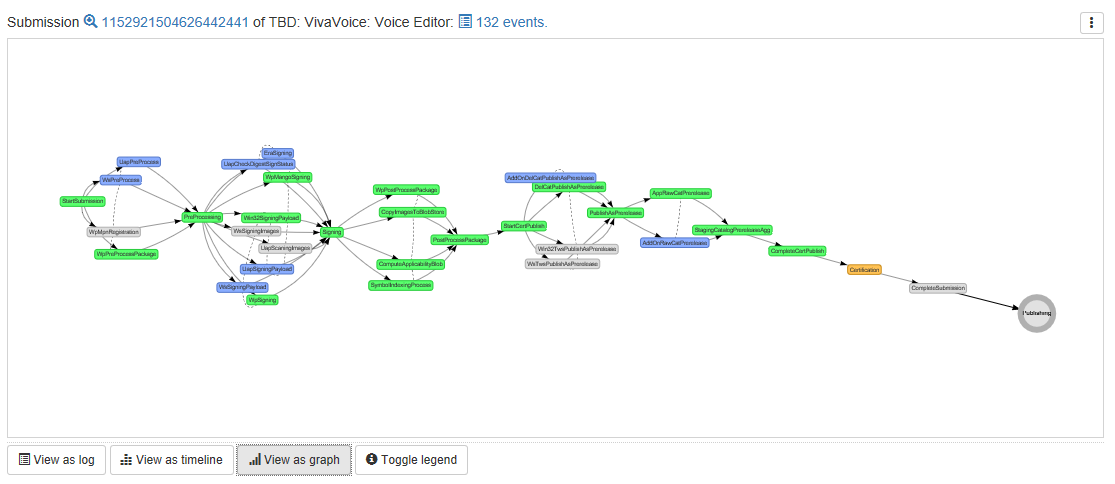
\includegraphics[width=\linewidth]{gfx/graph.png}
\caption{Graph view \label{fig:graph}}
\end{figure}

\begin{figure}[htb]
\centering 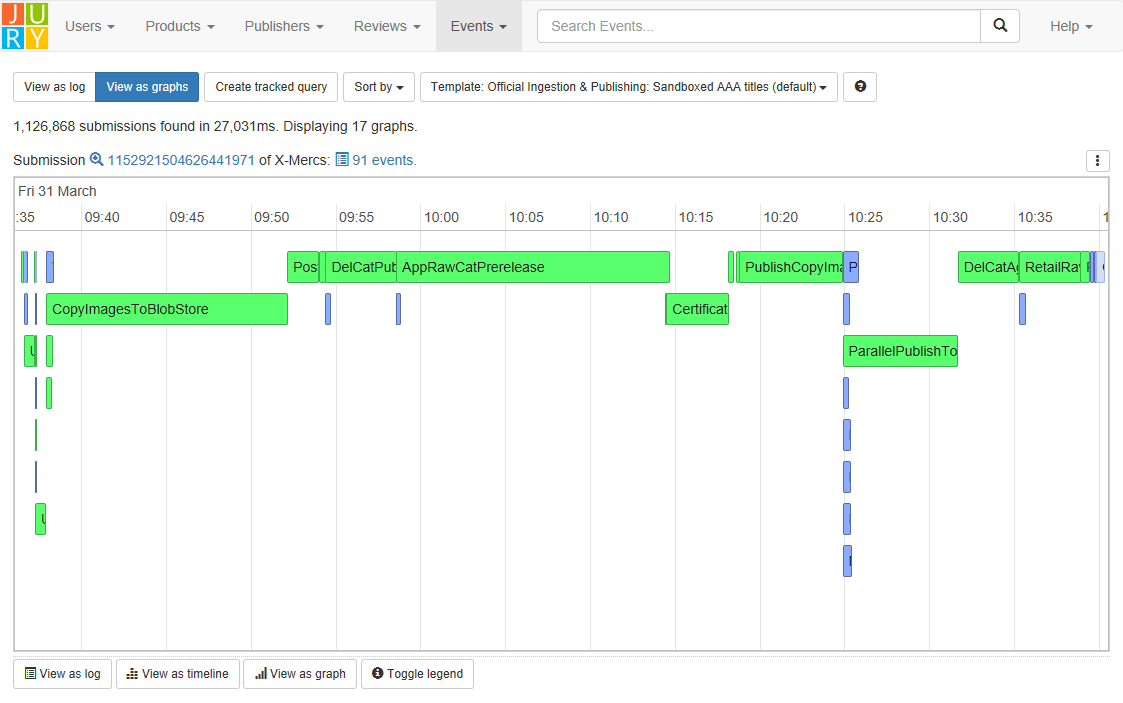
\includegraphics[width=\linewidth]{gfx/timeline.png}
\caption{Timeline view \label{fig:timeline}}
\end{figure}

\begin{figure}[htb]
\centering 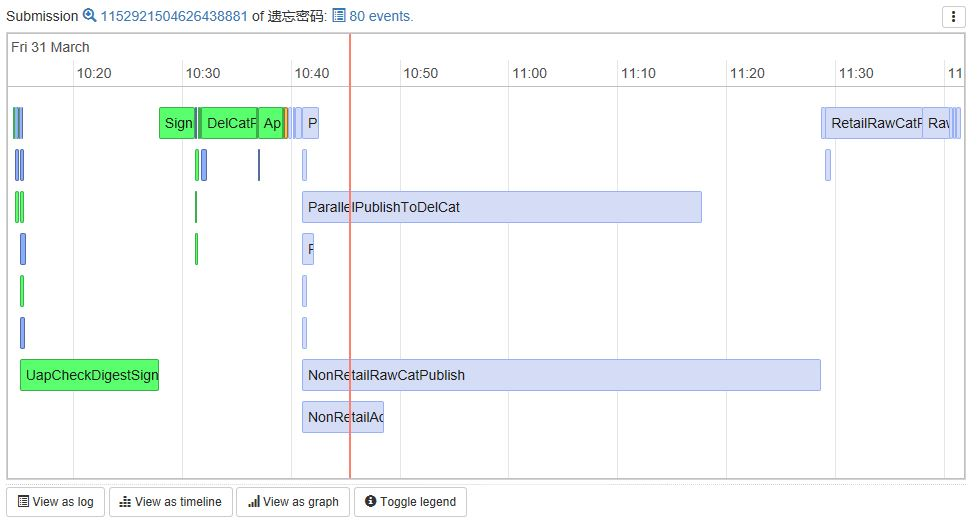
\includegraphics[width=\linewidth]{gfx/estimates.jpg}
\caption{Timeline view with estimates \label{fig:estimates}}
\end{figure}

\nyi{Statistics and their scores}
% (run stats on the same dataset)

\nyi{ML models and their scores}

\nyi{User satisfaction}

\subsection{Evaluation}
\label{sec:evaluation}

%Tutkimustuloksien merkityst\"a on aina syyt\"a arvioida ja tarkastella
%kriittisesti.  Joskus tarkastelu voi olla t\"ass\"a osassa, mutta se
%voidaan my\"os j\"att\"a\"a viimeiseen osaan, jolloin viimeisen osan nimeksi
%tulee >>Tarkastelu>>. Tutkimustulosten merkityst\"a voi arvioida my\"os
%>>Johtop\"a\"at\"okset>>-otsikon alla viimeisess\"a osassa. 

%T\"ass\"a osassa on syyt\"a my\"os arvioida tutkimustulosten luotettavuutta.
%Jos tutkimustulosten merkityst\"a arvioidaan >>Tarkastelu>>-osassa,
%voi luotettavuuden arviointi olla my\"os siell\"a. 

\nyi{Talk about success with graph generation}\\
\nyi{Maybe talk about alternative graph?}\\
\nyi{Changes in the system reflected real time (also a strength?)}\\
\nyi{Finding bugs in system (race conditions!) based on graphs}\\
\nyi{Feedback from users}

\nyi{Talk about negatives with machine learning models}\\
\nyi{Reason why they didn't end up working}

\nyi{Talk about how the system went immediately into production}\\
\nyi{Talk about the success of notifications built on top of the system}

%%%%%%%%%%%%%%%%%%%%%%%%%%%%%%%%%%%%%%%%%%%%%%%%%%%%%%%%%%%%%%%%%%%%%%%%%%%%%%%%

\subsection{Conclusions and Future Work} 
\label{sec:conclusions}

\begin{itemize}
\item[--]\nyi{Contributions (positives)}
\item[--]\nyi{Limitations (negatives)}
\item[--]\nyi{Future work}
\end{itemize}